\section{Consumer Headphones}
\label{sec:philipsphones}
There are many consumer noise cancelling headphones, which use various strategies to cancel the noise.
One of the cheaper versions available is Philips SHN2500.
Reverse engineering the circuit in these headphones reveals the schematic as shown in figure \ref{fig:philipsphonessche}.
Only one of two channels is shown in the schematic, the other channel is identical to the first, however shares components C25-27, and R31.
\\
\begin{sidewaysfigure}
	\centering
	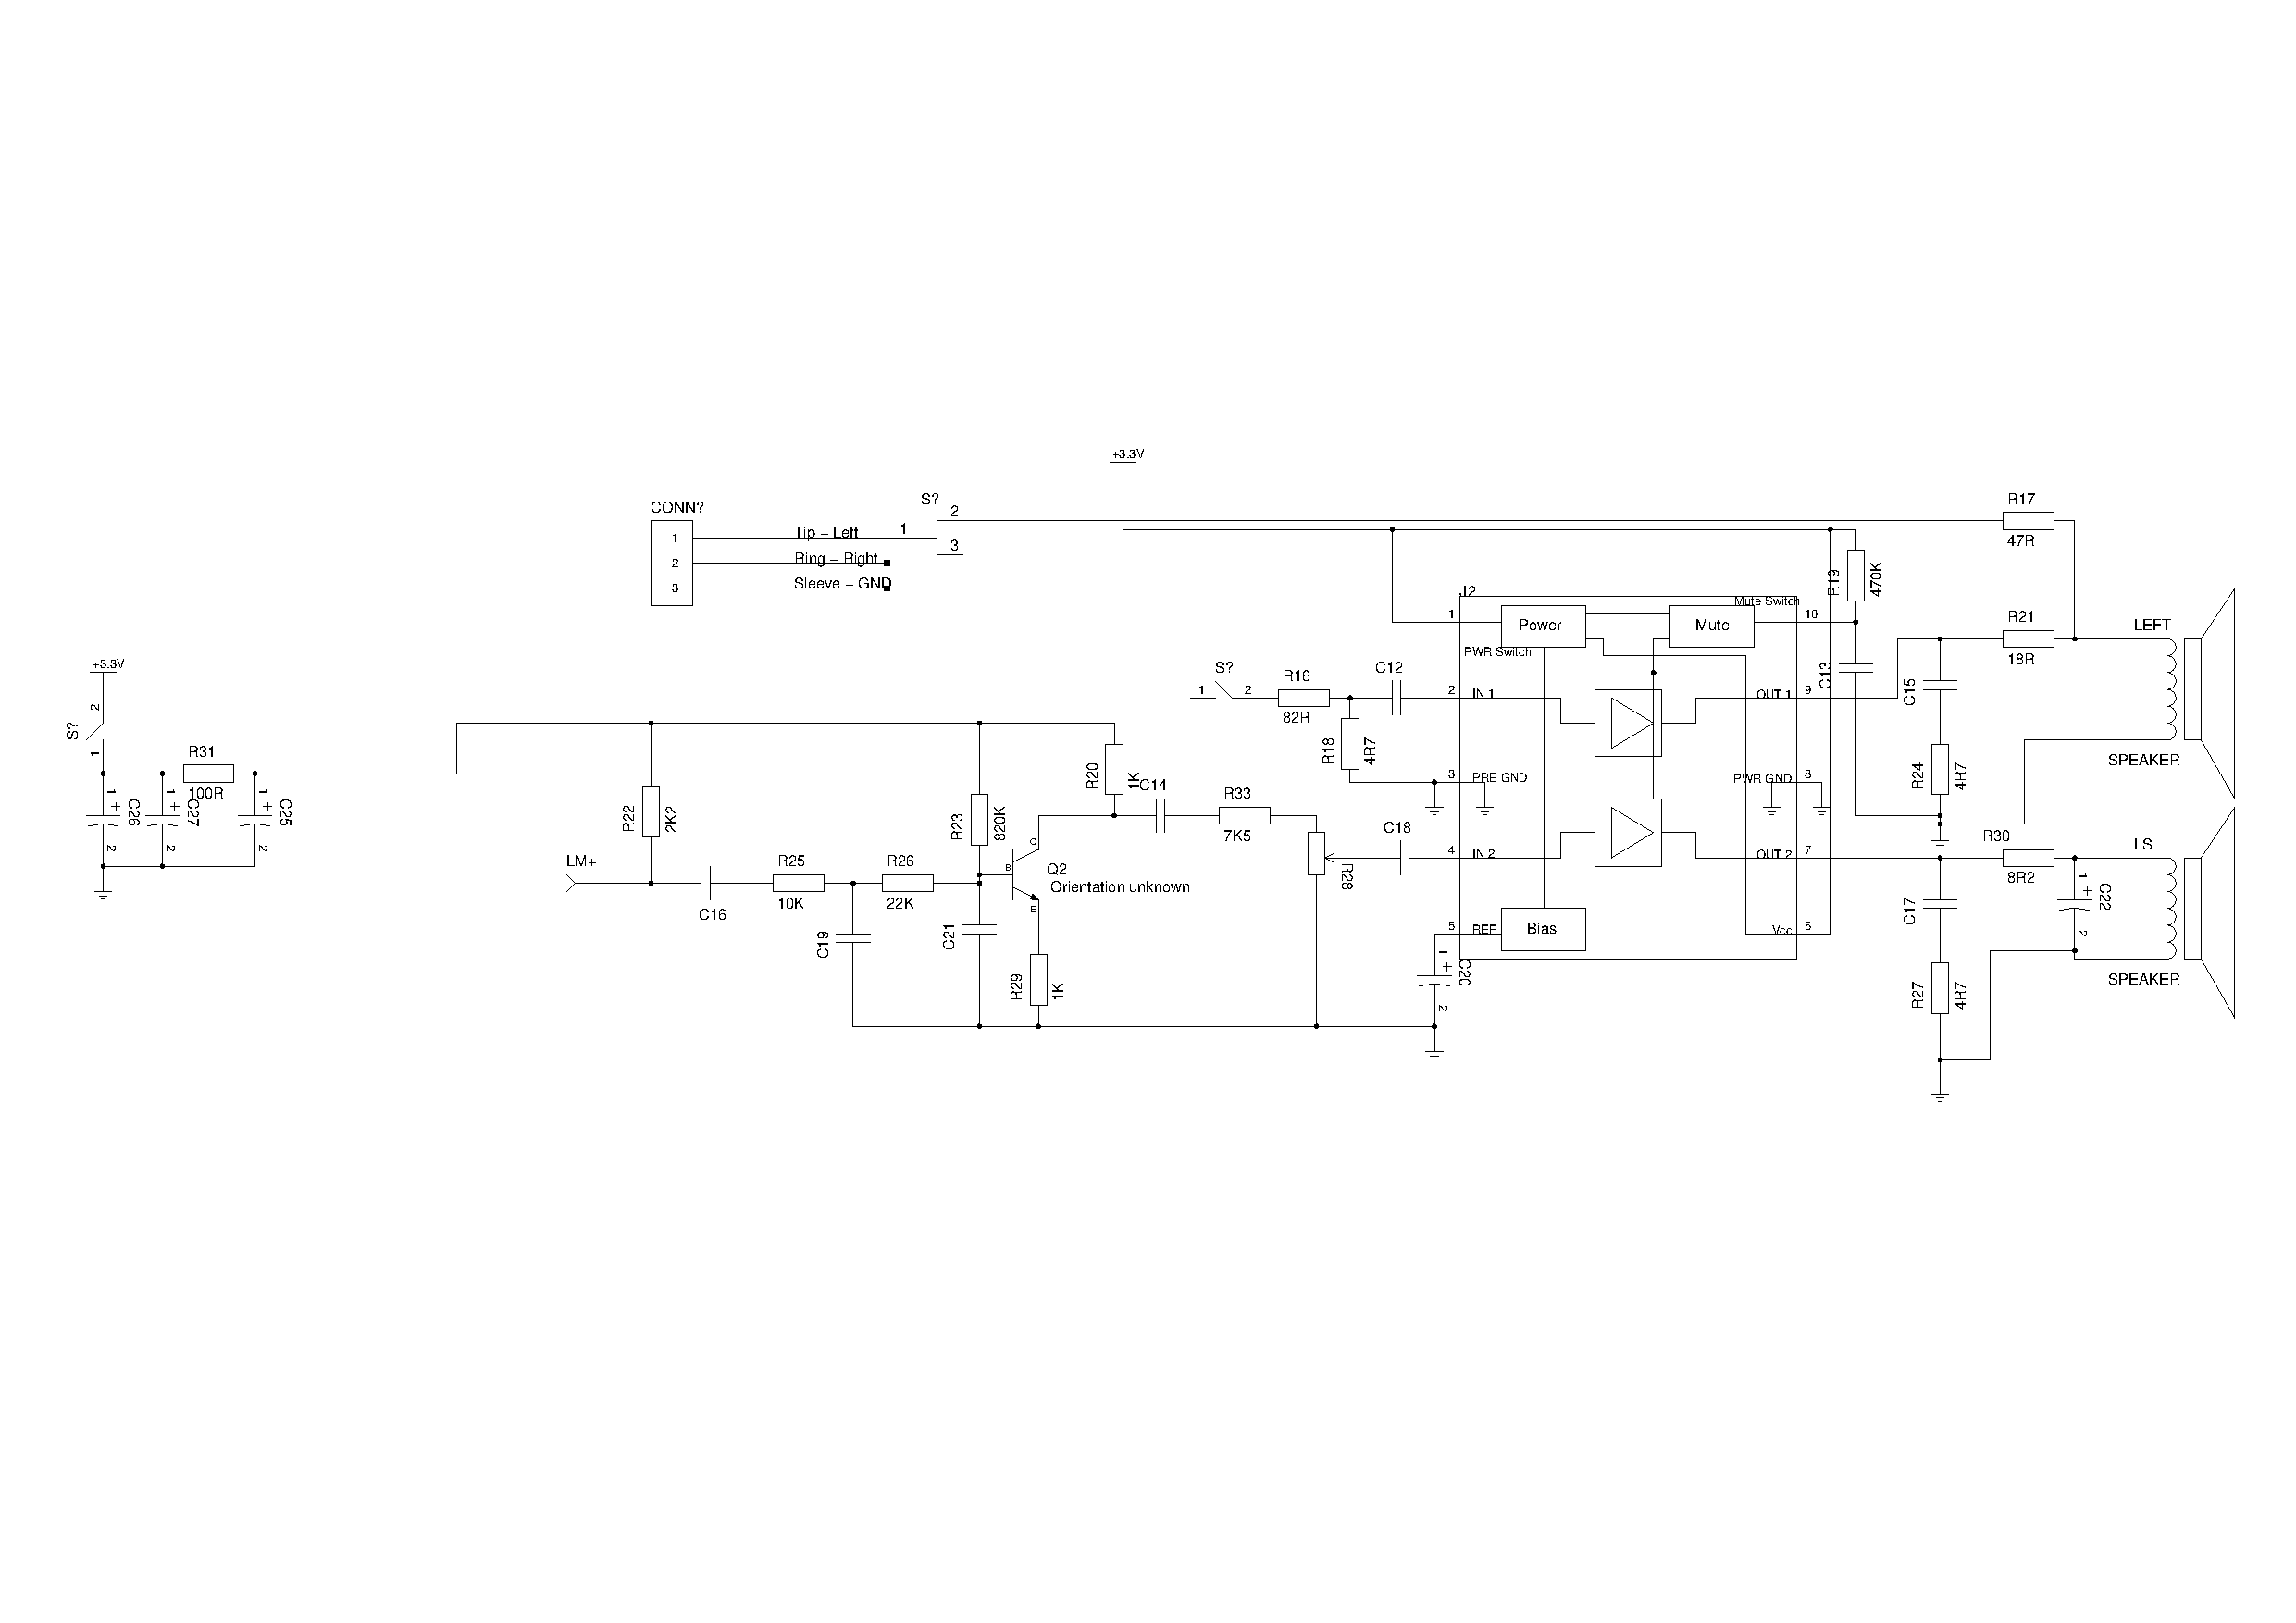
\includegraphics[width=\textwidth]{./img/hp.pdf}
	\caption{The reverse engineered schematic for the Philips SHN2500 Active Noise Cancelling Headphones}
	\label{fig:philipsphonessche}
\end{sidewaysfigure}

\noindent
There are two speakers inside the headphones; one of them carries the audio signal from the input device through to the ear.
The second one is driven by amplifier circuitry and forms the ANC portion of the headphones.
The noise signal arrives from a microphone built into the outside of the headphones; it then passes through a third order filter and amplifier stage.
The cancellation of the signal is achieved by the fact that the amplifier used at this point has a negative gain, therefore the signal produced will be anti-phase when compared to the sound heard.
The signals for both speakers then pass through a power amplifier and to the headphones.
\\
\\
The quality of the noise cancellation that these headphones provide is directly proportional to the price paid for them. They barely have any effect on the noise from the surroundings, and produce a slight hiss on top.
However, there is a lot to be said for the methodology of the system. By using an analogue system there is essentially no delay on the signal as it passes through, meaning that maximum cancellation can be achieved.
There is also minimal circuitry and component requirements, resulting in a low power draw, and low overheads in construction.
